\documentclass[12pt]{article}
\usepackage[utf8]{inputenc}
\usepackage{geometry}
\geometry{a4paper, margin=1in}
\usepackage{graphicx}
\usepackage{hyperref}
\usepackage[english]{babel}
\usepackage{pgfplots}
\usepackage{array}
\pgfplotsset{compat=1.18}

\title{Executive Report for Project 0003}
\author{Project Manager: Ana Silva}
\date{September 24, 2024}

\begin{document}

\maketitle

\tableofcontents
\newpage

\section*{Executive Summary}
\addcontentsline{toc}{section}{Executive Summary}
This report details the progress and current status of Project XYZ. It includes an analysis of the schedule, budget, and the main risks encountered. Additionally, strategies are presented to mitigate delays and improve team efficiency. The project, which began in June 2024, aims for completion by January 2025.

\section*{Context}
\addcontentsline{toc}{section}{Context}
Project XYZ was created to modernize the company’s IT infrastructure, focusing on the implementation of a new data management system. The main goal is to reduce data processing time by 40% and enhance data security. The project team includes IT specialists, software engineers, and external consultants.

The key objectives include:
\begin{itemize}
    \item Reduce data processing time by 40%.
    \item Implement an automated backup system.
    \item Enhance security with advanced encryption.
    \item Improve data accessibility for different departments.
\end{itemize}

\section*{Progress To Date}
\addcontentsline{toc}{section}{Progress To Date}
The project is currently in the development phase, with 70\% of the tasks completed. Below is a summary of the finished stages:

\begin{itemize}
    \item \textbf{Phase 1: Planning and Design} (Completed on July 30, 2024)
    \item \textbf{Phase 2: Development} (70\% complete, expected completion by October 20, 2024)
    \item \textbf{Phase 3: Testing and Deployment} (Scheduled for November-December 2024)
\end{itemize}

\section*{Project Schedule and Milestones}
\addcontentsline{toc}{section}{Project Schedule and Milestones}
The following table shows the detailed schedule of the project’s milestones and the completion status of each:

\begin{center}
\begin{tabular}{|m{4cm}|m{3cm}|m{3cm}|m{3cm}|}
\hline
\textbf{Milestone} & \textbf{Planned Date} & \textbf{Actual Date} & \textbf{Completion Status} \\
\hline
Planning Complete & July 30, 2024 & July 30, 2024 & 100\% \\
\hline
API Development & September 15, 2024 & September 20, 2024 & 100\% \\
\hline
Database Integration & October 1, 2024 & In progress & 60\% \\
\hline
System Testing & November 15, 2024 & To be defined & Not Started \\
\hline
Final Deployment & January 15, 2025 & To be defined & Not Started \\
\hline
\end{tabular}
\end{center}

\section*{Budget Analysis}
\addcontentsline{toc}{section}{Budget Analysis}
The project budget is within limits, although delays in database integration may result in additional costs. Below is the allocated budget compared to actual spending to date:

\begin{itemize}
    \item \textbf{Total Budget:} R\$600,000
    \item \textbf{Total Spent:} R\$350,000 (As of September 24, 2024)
\end{itemize}

\subsection*{Budget Breakdown}
\begin{itemize}
    \item Planning and Design: R\$120,000 (Spent: R\$110,000)
    \item Development: R\$300,000 (Spent: R\$180,000)
    \item Testing: R\$120,000 (Allocated)
    \item Deployment: R\$60,000 (Allocated)
\end{itemize}

\section*{Current Status}
\addcontentsline{toc}{section}{Current Status}
The project is currently focused on database integration. Below is a Gantt chart illustrating the project schedule:

\begin{center}
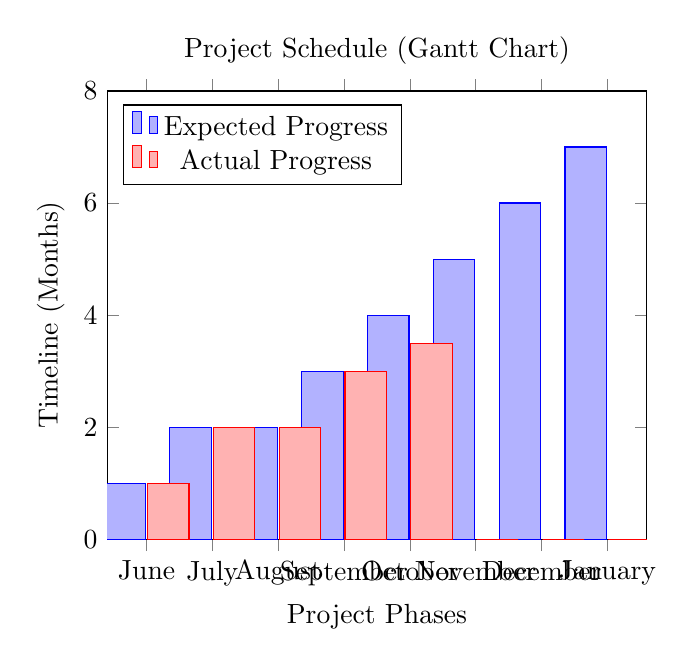
\begin{tikzpicture}
    \begin{axis}[
        title={Project Schedule (Gantt Chart)},
        xlabel={Project Phases},
        ylabel={Timeline (Months)},
        symbolic x coords={June, July, August, September, October, November, December, January},
        xtick=data,
        ybar=0.7,
        ymin=0, ymax=8,
        bar width=15pt,
        enlarge x limits={abs=0.5cm},
        legend pos=north west
    ]
    \addplot coordinates {(June, 1) (July, 2) (August, 2) (September, 3) (October, 4) (November, 5) (December, 6) (January, 7)};
    \addlegendentry{Expected Progress}
    
    \addplot coordinates {(June, 1) (July, 2) (August, 2) (September, 3) (October, 3.5) (November, 0) (December, 0) (January, 0)};
    \addlegendentry{Actual Progress}
    \end{axis}
\end{tikzpicture}
\end{center}

\section*{Risks and Mitigation}
\addcontentsline{toc}{section}{Risks and Mitigation}
Some identified risks that may impact the project’s schedule and budget include:
\begin{itemize}
    \item \textbf{Risk:} Delays in database integration.
    \item \textbf{Mitigation:} Allocate a dedicated team to accelerate the integration process.
    \item \textbf{Risk:} Security issues during testing.
    \item \textbf{Mitigation:} Implement continuous security audits during development.
\end{itemize}

\section*{Next Steps}
\addcontentsline{toc}{section}{Next Steps}
The key activities for the next few weeks are:
\begin{itemize}
    \item Finalize database integration by October 15, 2024.
    \item Start system testing by November 1, 2024.
    \item Ensure deployment is completed by January 2025.
\end{itemize}

\section*{Conclusion}
\addcontentsline{toc}{section}{Conclusion}
Project XYZ is progressing according to the revised schedule. Although there have been delays in development, the additional resources allocated should ensure the project is completed within the revised deadline. It is expected that the database integration will be completed soon, allowing system testing and deployment to proceed as planned.

\end{document}
